%%%%%%%%%%%%%%%%%%%%%%% file template.tex %%%%%%%%%%%%%%%%%%%%%%%%%
%
% This is a template file for the LaTeX package SVJour2 for the
% Springer journal "The VLDB Journal".
%
%                                    Springer Heidelberg 2004/12/03
%
% Copy it to a new file with a new name and use it as the basis
% for your article. Delete % as needed.
%
%%%%%%%%%%%%%%%%%%%%%%%%%%%%%%%%%%%%%%%%%%%%%%%%%%%%%%%%%%%%%%%%%%%
%
% First comes an example EPS file -- just ignore it and
% proceed on the \documentclass line
% your LaTeX will extract the file if required
%\begin{filecontents*}{figs/minimalperfecthash-ph-mph.ps}
%!PS-Adobe-3.0 EPSF-3.0
%%BoundingBox: 19 19 221 221
%%CreationDate: Mon Sep 29 1997
%%Creator: programmed by hand (JK)
%%EndComments
%gsave
%newpath
%  20 20 moveto
%  20 220 lineto
%  220 220 lineto
%  220 20 lineto
%closepath
%2 setlinewidth
%gsave
%  .4 setgray fill
%grestore
%stroke
%grestore
%\end{filecontents*}
%
\documentclass[twocolumn,fleqn,runningheads]{svjour2}
%
\smartqed  % flush right qed marks, e.g. at end of proof
%
\usepackage{graphicx}
\usepackage{listings}
%
% \usepackage{mathptmx}      % use Times fonts if available on your TeX system
%
% insert here the call for the packages your document requires
%\usepackage{latexsym}
% etc.
%
% please place your own definitions here and don't use \def but
% \newcommand{}{}
%

\lstset{
  language=Pascal,
  basicstyle=\fontsize{9}{9}\selectfont,
  captionpos=t,
  aboveskip=1mm,
  belowskip=1mm,
  abovecaptionskip=1mm,
  belowcaptionskip=1mm,
%  numbers = left,
  mathescape=true,
  escapechar=@,
  extendedchars=true,
  showstringspaces=false,
  columns=fixed,
  basewidth=0.515em,
  frame=single,
  framesep=2mm,
  xleftmargin=2mm,
  xrightmargin=2mm,
  framerule=0.5pt
}

\def\cG{{\mathcal G}}
\def\crit{{\rm crit}}
\def\ncrit{{\rm ncrit}}
\def\scrit{{\rm scrit}}
\def\bedges{{\rm bedges}}
\def\ZZ{{\mathbb Z}}

\journalname{The VLDB Journal}
%
\begin{document}

\title{Minimal Perfect Hash Functions: New Algorithms and Applications\thanks{
This work was supported in part by
GERINDO Project--grant MCT/CNPq/CT-INFO 552.087/02-5,
CAPES/PROF Scholarship (Fabiano C. Botelho),
FAPESP Proj.\ Tem.\ 03/09925-5 and CNPq Grant 30.0334/93-1
(Yoshiharu Kohayakawa),
and CNPq Grant 30.5237/02-0 (Nivio Ziviani).}
}
%\subtitle{Do you have a subtitle?\\ If so, write it here}

%\titlerunning{Short form of title}        % if too long for running head

\author{Fabiano C. Botelho \and Davi C. Reis \and Yoshiharu Kohayakawa \and Nivio Ziviani}
%\authorrunning{Short form of author list} % if too long for running head
\institute{
F. C. Botelho \and 
N. Ziviani \at
Dept. of Computer Science,
Federal Univ. of Minas Gerais,
Belo Horizonte, Brazil\\
\email{\{fbotelho,nivio\}@dcc.ufmg.br}
\and
D. C. Reis \at
Google, Brazil \\
\email{davi.reis@gmail.com}
\and
Y. Kohayakawa
Dept. of Computer Science,
Univ. of S\~ao Paulo,
S\~ao Paulo, Brazil\\
\email{yoshi@ime.usp.br}
}

\date{Received: date / Accepted: date}
% The correct dates will be entered by the editor


\maketitle

\begin{abstract}
Insert your abstract here. Include up to five keywords.
\keywords{First keyword \and Second keyword \and More}
\end{abstract}

% main text
\section{Introduction} \label{sec:introduction}


The important performance parameters of a PHF are representation size, evaluation time and construction time. The representation size plays an important role when the whole function fits in a faster memory and the actual data is stored in a slower memory. For instace, compact PHFs can be entirely fit in a CPU cache and this makes their computation really fast by avoiding cache misses. The CHD algorithm plays an important role in this context. It was designed by Djamal Belazzougui, Fabiano C. Botelho, and Martin Dietzfelbinger in \cite{bbd09}.


The CHD algorithm permits to obtain PHFs with representation size very close to optimal while retaining $O(n)$ construction time and $O(1)$ evaluation time. For example, in the case $m=2n$ we obtain a PHF that uses space $0.67$ bits per key, and for $m=1.23n$ we obtain space $1.4$ bits per key, which was not achievable with previously known methods. The CHD algorithm is inspired by several known algorithms; 
the main new feature is that it combines a modification of Pagh's ``hash-and-displace'' approach
with data compression on a sequence of hash function indices. 
That combination makes it possible to significantly reduce space usage 
while retaining linear construction time and constant query time. 
The CHD algorithm can also be used for $k$-perfect hashing,
where at most $k$ keys may be mapped to the same value.
For the analysis we assume that fully random hash functions are given for free;
such assumptions can be justified and were made in previous papers.

The compact PHFs generated by the CHD algorithm can be used in many applications in which we want to assign a unique identifier to each key without storing any information on the key. One of the most obvious applications of those functions 
(or $k$-perfect hash functions) is when we have a small fast memory in which we can store the perfect hash function while the keys and associated satellite data are stored in slower but larger memory. 
The size of a block or a transfer unit may be chosen so that $k$ data items can be retrieved in
one read access. In this case we can ensure that data associated with a key can be retrieved in a single probe to slower memory. This has been used for example in hardware routers~\cite{pb06}. 
% Perfect hashing has also been found to be competitive with traditional hashing in internal memory~\cite{blmz08} on standard computers. Recently perfect hashing has been used to accelerate algorithms on graphs~\cite{ESS08} when the graph representation does not fit in main memory.


The CHD algorithm generates the most compact PHFs and MPHFs we know of in~$O(n)$ time. 
The time required to evaluate the generated functions is constant (in practice less than $1.4$ microseconds). 
The storage space of the resulting PHFs and MPHFs are distant from the information 
theoretic lower bound by a factor of $1.43$.
The closest competitor is the algorithm by Martin and Pagh \cite{dp08} but
their algorithm do not work in linear time.
Furthermore, the CHD algorithm 
can be tuned to run faster than the BPZ algorithm \cite{bpz07} (the fastest algorithm
available in the literature so far) and to obtain more compact functions.
The most impressive characteristic is that it has the ability, in principle, to
approximate the information theoretic lower bound while being practical.
A detailed description of the CHD algorithm can be found in \cite{bbd09}. 




\section{Related Work}
Czech, Havas and Majewski~\cite{chm97} provide a
comprehensive survey of the most important theoretical results
on perfect hashing.
In the following, we review some of those results.

Fredman, Koml\'os and Szemer\'edi~\cite{FKS84} showed that it is possible to
construct space efficient perfect hash functions that can be evaluated in
constant time with table sizes that are linear in the number of keys:
$m=O(n)$.  In their model of computation, an element of the universe~$U$ fits
into one machine word, and arithmetic operations and memory accesses have unit
cost.  Randomized algorithms in the FKS model can construct a perfect hash
function in expected time~$O(n)$:
this is the case of our algorithm and the works in~\cite{chm92,p99}.

Many methods for generating minimal perfect hash functions use a
{\em mapping}, {\em ordering} and {\em searching}
(MOS) approach,
a description coined by Fox, Chen and Heath~\cite{fch92}.
In the MOS approach, the construction of a minimal perfect hash function
is accomplished in three steps.
First, the mapping step transforms the key set from the original universe
to a new universe.
Second, the ordering step places the keys in a sequential order that
determines the order in which hash values are assigned to keys.
Third, the searching step attempts to assign hash values to the keys.
Our algorithm and the algorithm presented in~\cite{chm92} use the
MOS approach.

Pagh~\cite{p99} proposed a family of randomized algorithms for
constructing minimal perfect hash functions.
The form of the resulting function is $h(x) = (f(x) + d_{g(x)}) \bmod n$,
where $f$ and $g$ are universal hash functions and $d$ is a set of
displacement values to resolve collisions that are caused by the function $f$.
Pagh identified a set of conditions concerning $f$ and $g$ and showed
that if these conditions are satisfied, then a minimal perfect hash
function can be computed in expected time $O(n)$ and stored in
$(2+\epsilon)n$ computer words.
Dietzfelbinger and Hagerup~\cite{dh01} improved~\cite{p99},
reducing from $(2+\epsilon)n$ to $(1+\epsilon)n$ the number of computer
words required to store the function, but in their approach~$f$ and~$g$ must
be chosen from a class
of hash functions that meet additional requirements.
Differently from the works in~\cite{p99,dh01}, our algorithm uses two
universal hash functions $h_1$ and $h_2$ randomly selected from a class
of universal hash functions that do not need to meet any additional
requirements.

The work in~\cite{chm92} presents an efficient and practical algorithm
for generating order preserving minimal perfect hash functions.
Their method involves the generation of acyclic random graphs
$G = (V, E)$ with~$|V|=cn$ and $|E|=n$, with  $c \ge 2.09$.
They showed that an order preserving minimal perfect hash function
can be found in optimal time if~$G$ is acyclic.
To generate an acyclic graph, two vertices $h_1(x)$ and $h_2(x)$ are
computed for each key $x \in S$.
Thus, each set~$S$ has a corresponding graph~$G=(V,E)$, where $V=\{0,1,
\ldots,t\}$ and $E=\big\{\{h_1(x),h_2(x)\}:x \in S\big\}$.
In order to guarantee the acyclicity of~$G$, the algorithm repeatedly selects
$h_1$ and $h_2$ from a family of universal hash functions
until the corresponding graph is acyclic.
Havas et al.~\cite{hmwc93} proved that if $|V(G)|=cn$ and $c>2$,
then the probability that~$G$ is acyclic is $p=e^{1/c}\sqrt{(c-2)/c}$.
For $c=2.09$, this probability is
$p \simeq 0.342$, and
the expected number of iterations to obtain an acyclic graph
is~$1/p \simeq 2.92$.
\section{Os Algoritmos}
\label{sec:thealgorithm}

\subsection{Um Algoritmo Baseado em Mem\'oria Principal}

\subsection{Um Algoritmo Baseado em Mem\'oria Externa}
% For two-column wide figures use
\begin{figure}
% Use the relevant command to insert your figure file.
% For example, with the graphicx package use
\centering
  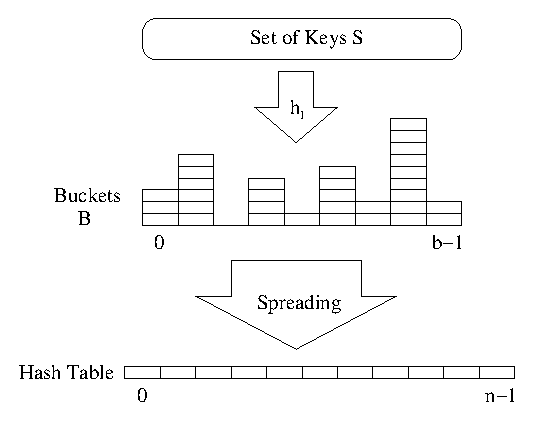
\includegraphics{figs/brz.ps}
% figure caption is below the figure
\caption{Main steps of the new algorithm.}
\label{fig:new-algo-main-steps}
\end{figure}

\subsubsection{Segmenta\c{c}\~ao}
\subsubsection{Espalhamento}

\section{Experimental Results}

% We now present some experimental results.
% The same experiments were run with our algorithm and
% the algorithm due to Czech, Havas and Majewski~\cite{chm92}, referred to as
% the CHM algorithm.
% The two algorithms were implemented in the C language and
% are available at \texttt{http://cmph.sf.net}.
% Our data consists
% of a collection of 100 million
% universe resource locations (URLs) collected from the Web.
% The average length of a URL in the collection is 63 bytes.
% All experiments were carried out on
% a computer running the Linux operating system, version 2.6.7,
% with a 2.4 gigahertz processor and
% 4 gigabytes of main memory.
% 
% Table~\ref{tab:characteristics} presents the main characteristics
% of the two algorithms.
% The number of edges in the graph $G=(V,E)$ is~$|S|=n$,
% the number of keys in the input set~$S$.
% The number of vertices of $G$ is equal to $1.15n$ and $2.09n$
% for our algorithm and the CHM algorithm, respectively.
% This measure is related to the amount of space to store the array $g$.
% This improves the space required to store a function in our algorithm to
% $55\%$ of the space required by the CHM algorithm.
% The number of critical edges
% is $\frac{1}{2}|E(G)|$ and 0 for our algorithm and the CHM algorithm,
% respectively.
% Our algorithm generates random graphs that contain cycles with high
% probability and the
% CHM algorithm
% generates
% acyclic random graphs.
% Finally, the CHM algorithm generates order preserving functions
% while our algorithm does not preserve order.
% 
% \vspace{-10pt}
% \begin{table}[htb]
% {\footnotesize 
% \begin{center}
% \begin{tabular}{|c|c|c|c|c|c|c|}
% \hline
%                  & $c$  & $|E(G)|$ & $|V(G)|=|g|$ & $|E(G_\crit)|$ & $G$     & Order preserving \\
% \hline
% Our  algorithm   & 1.15 & $n$      & $cn$         & $0.5|E(G)|$    & cyclic  & no \\
% \hline
% CHM  algorithm   & 2.09 & $n$      & $cn$         & 0              & acyclic & yes \\
% \hline
% \end{tabular}
% \end{center}
% }
% \caption{Main characteristics of the algorithms}
% \vspace{-25pt}
% \label{tab:characteristics}
% \end{table}
% 
% Table~\ref{tab:timeresults} presents time measurements.
% All times are in seconds.
% The table entries are averages over 50 trials.
% The column labelled $N_i$ gives
% the number of iterations to generate the random graph $G$
% in the mapping step of the algorithms.
% The next columns give the running times
% for the mapping plus ordering steps together and the searching
% step for each algorithm.
% The last column gives the percentage gain of our algorithm
% over the CHM algorithm.
% 
% \begin{table*}
% {\footnotesize 
% \begin{center}
% \begin{tabular}{|c|cccc|cccc|c|}
% \hline 
% \raisebox{-0.7em}{$n$} & \multicolumn{4}{c|}{\raisebox{-1mm}{Our algorithm}} &
% \multicolumn{4}{c|}{\raisebox{-1mm}{CHM algorithm}}& \raisebox{-0.2em}{Gain}\\
% \cline{2-5} \cline{6-9} 
%  & \raisebox{-1mm}{$N_i$} &\raisebox{-1mm}{Map+Ord} &
% \raisebox{-1mm}{Search} &\raisebox{-1mm}{Total}  &
% \raisebox{-1mm}{$N_i$} &\raisebox{-1mm}{Map+Ord} &\raisebox{-1mm}{Search} &
% \raisebox{-1mm}{Total} & \raisebox{0.2em}{(\%)}\\
% \hline
% %1,562,500    & 2.28 & 8.54   & 2.37   & 10.91   & 2.70 & 14.56    & 1.57   & 16.13    & 48 \\ %[1mm]
% %3,125,000    & 2.16 & 15.92  & 4.88   & 20.80   & 2.85 & 30.36    & 3.20   & 33.56    & 61 \\ %[1mm]
% 6,250,000    & 2.20 & 33.09  & 10.48  & 43.57   & 2.90 & 62.26    & 6.76   & 69.02    & 58 \\ %[1mm]
% 12,500,000   & 2.00 & 63.26  & 23.04  & 86.30   & 2.60 & 117.99   & 14.94  & 132.92   & 54 \\ %[1mm]
% 25,000,000   & 2.00 & 130.79 & 51.55  & 182.34  & 2.80 & 262.05   & 33.68  & 295.73   & 62 \\ %[1mm]
% %50,000,000   & 2.07 & 273.75 & 114.12 & 387.87  & 2.90 & 577.59   & 73.97  & 651.56   & 68 \\ %[1mm]
% 100,000,000  & 2.07 & 567.47 & 243.13 & 810.60  & 2.80 & 1,131.06 & 157.23 & 1,288.29 & 59 \\ %[1mm]
% \hline
% \end{tabular}
% \end{center}
% \caption{Time measurements
% for our algorithm and the CHM algorithm}
% \vspace{-25pt}
% \label{tab:timeresults}
% }\end{table*}
% 
% \enlargethispage{\baselineskip}
% The mapping step of the new algorithm is faster because
% the expected number of iterations in the mapping step to generate
% $G$ are 2.13 and 2.92 for our algorithm and the CHM algorithm, respectively.
% The graph $G$ generated by our algorithm
% has $1.15n$ vertices, against $2.09n$ for the CHM algorithm.
% These two facts make our algorithm faster in the mapping step.
% The ordering step of our algorithm is approximately equal to
% the time to check if $G$ is acyclic for the CHM algorithm.
% The searching step of the CHM algorithm is faster, but the total
% time of our algorithm is, on average, approximately 58\% faster
% than the CHM algorithm.
% 
% The experimental results fully backs the theoretical results.
% It is important to notice the times for the searching step:
% for both algorithms they are not the dominant times,
% and the experimental results clearly show
% a linear behavior for the searching step.
% 
% We now present a heuristic that reduces the space requirement
% to any given value between $1.15n$ words and $0.93n$ words.
% The heuristic reuses, when possible, the set
% of $x$ values that caused reassignments, just before trying $x+1$
% (see Section~\ref{sec:searching}).
% The lower limit $c=0.93$ was obtained experimentally. 
% We generate $10{,}000$ random graphs for 
% each size $n$ ($n=10^5$, $5 \times 10^5$, $10^6$, $2\times 10^6$). 
% With $c=0.93$ we were always able to generate~$h$, but with $c=0.92$ we never
% succeeded.
% Decreasing the value of $c$ leads to an increase in the number of
% iterations to generate $G$.
% For example, for $c=1$ and $c=0.93$, the analytical expected number
% of iterations are $2.72$ and $3.17$, respectively
% (for $n=12{,}500{,}000$, the number of iterations are 2.78 for $c=1$ and 3.04
% for $c=0.93$).
% Table~\ref{tab:timeresults2} presents the total times to construct a
% function for $n=12{,}500{,}000$, with an increase from $86.31$ seconds
% for $c=1.15$ (see Table~\ref{tab:timeresults}) to
% $101.74$ seconds for $c=1$ and to $102.19$ seconds for $c=0.93$.
% 
% \vspace{-5pt}
% \begin{table*}
% {\footnotesize 
% \begin{center}
% \begin{tabular}{|c|cccc|cccc|}
% \hline 
% \raisebox{-0.7em}{$n$} & \multicolumn{4}{c|}{\raisebox{-1mm}{Our algorithm $c=1.00$}} &
% \multicolumn{4}{c|}{\raisebox{-1mm}{Our algorithm $c=0.93$}} \\
% \cline{2-5} \cline{6-9}
%  & \raisebox{-1mm}{$N_i$} &\raisebox{-1mm}{Map+Ord} &
% \raisebox{-1mm}{Search} &\raisebox{-1mm}{Total}  &
% \raisebox{-1mm}{$N_i$} &\raisebox{-1mm}{Map+Ord} &\raisebox{-1mm}{Search} &
% \raisebox{-1mm}{Total} \\%[0.3mm]
% \hline%\\[-2mm]
% 12,500,000   & 2.78 & 76.68  & 25.06  & 101.74  & 3.04 & 76.39   & 25.80  & 102.19 \\ %[1mm]
% \hline
% \end{tabular}
% \end{center}
% \caption{Time measurements
% for our tuned algorithm with $c=1.00$ and $c=0.93$}
% \vspace{-25pt}
% \label{tab:timeresults2}
% }
% \end{table*}
% 
% We compared our algorithm with the ones proposed by Pagh~\cite{p99} and 
% Dietzfelbinger and Hagerup~\cite{dh01}, respectively. The authors sent to us their 
% source code. In their implementation the set of keys is a set of random integers. 
% We modified our implementation to generate our~$h$ from a set of random 
% integers in order to make a fair comparison. For a set of $10^6$ random integers,
% the times to generate a minimal perfect hash function were $2.7 s$, $4 s$ and $4.5 s$ for
% our algorithm, Pagh's algorithm and Dietzfelbinger and Hagerup's algorithm, respectively.
% Thus, our algorithm was 48\% faster than Pagh's algorithm and 67\% faster than
% Dietzfelbinger and Hagerup's algorithm, on average. This gain was maintained for sets with different
% sizes. 
% Our algorithm needs $kn$ ($k \in [0.93, 1.15]$) words to store 
% the resulting function, while Pagh's algorithm needs $kn$ ($k > 2$) words and 
% Dietzfelbinger and Hagerup's algorithm needs $kn$ ($k \in [1.13, 1.15]$) words. 
% The time to generate the functions is inversely proportional to the value of $k$.
% \enlargethispage{\baselineskip}

\section{Applications}
\label{sec:applications}
\section{Conclus\~oes}





%\begin{acknowledgements}
%If you'd like to thank anyone, place your comments here
%and remove the percent signs.
%\end{acknowledgements}

% BibTeX users please use
%\bibliographystyle{spmpsci}
%\bibliography{}   % name your BibTeX data base
\bibliographystyle{plain}
\bibliography{references}
\end{document}
